\documentclass[tikz, border=10pt]{standalone}

\usepackage{tikz}

\begin{document}

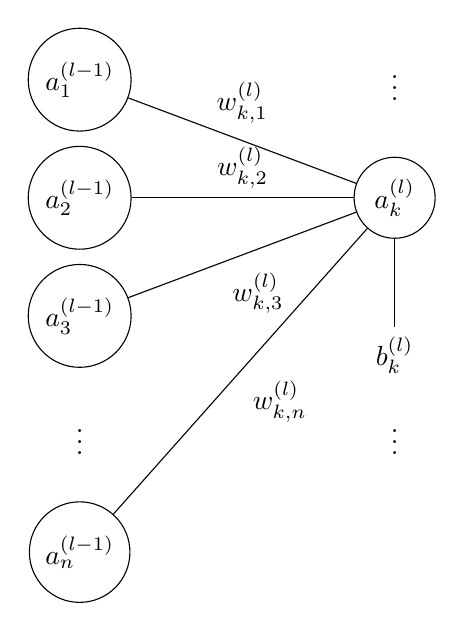
\begin{tikzpicture}[
    neuron/.style={circle, draw, minimum size=1cm}
]

    \foreach \i in {1,...,3}
        \node[neuron] (L\i) at (0,-\i*1.5) {$a_{\i}^{(l-1)}$};

    \node at (0, {-4*1.5}) {\vdots};

    \node[neuron] (L4) at (0,-5*1.5) {$a_{n}^{(l-1)}$};

    \node at (4, -1.5) {\vdots};

    \node[neuron] (O) at (4, -3) {$a_{k}^{(l)}$};

    \node at (4, {-4*1.5}) {\vdots};

    \node (B) at (4, -5) {$b^{(l)}_k$};

    \draw (L1) --node[midway, above, yshift=0.1cm] {$w_{k,1}^{(l)}$} (O);
    \draw (L2) --node[midway, above] {$w_{k,2}^{(l)}$} (O);
    \draw (L3) --node[midway, below, xshift=0.2cm, yshift=-0.1cm] {$w_{k,3}^{(l)}$} (O);
    \draw (L4) --node[midway, below, xshift=0.5cm] {$w_{k,n}^{(l)}$} (O);

    \draw (B) -- (O);

\end{tikzpicture}

\end{document}
